\vspace{-5px}\section{Introduction}\label{sect:intro}\vspace{-5px}

\begin{figure}[t]
    \centering
    \vspace{-20px}
    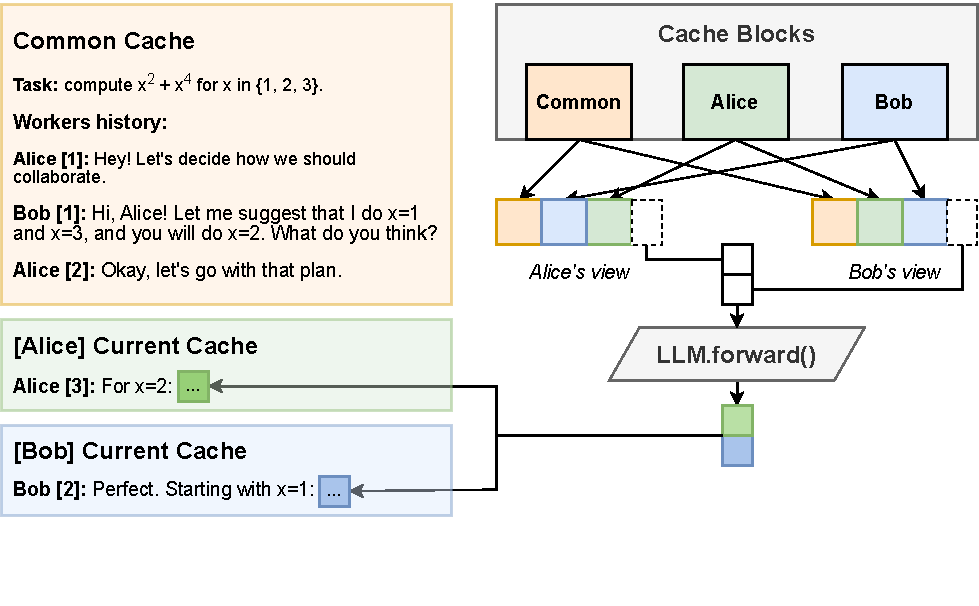
\includegraphics[width=0.9\linewidth, height=215px]{resources/figure1_cropped.pdf}\vspace{-20px}
    \caption{An intuitive explanation of Hogwild!\! Inference, with 2 workers generating in parallel and 3 shared cache blocks. Each color denotes a cache block. \href{https://github.com/eqimp/hogwild_llm/tree/main?tab=readme-ov-file\#demo}{See it in action (example generation)}.}
    \label{fig:teaser}\vspace{-20px}
\end{figure}

A recent trend allowing for further progress in Large Language Models is to leverage their ability to improve performance via additional inference-time computations~\citep{challenging_bigbench_solved_with_cot_Suzgun2022ChallengingBT,scaling_test_time_snell2024scaling,beeching2024scalingtesttimecompute,muennighoff2025s1}. This includes improved reasoning~\citep{cot_wei_2022,zero_shot_cot_Kojima2022LargeLM,auto_cot_Zhang2022AutomaticCO,three_of_thought,verify_step_by_step}, long-form generation~\citep{Bai2024LongWriterU1} and interacting with external tools~\citep{Schick2023ToolformerLM,Qin2023ToolLLMFL,Yao2022ReActSR,Shen2023HuggingGPTSA}. Modern LLM-based services have capabilities for long-form reasoning~\citep{openai_o1,googledeepmind2025gemini25thinking,AnthropicClaude3.7Sonnet}. At the same time, several highly capable reasoning LLMs have recently been released to the public ~\cite{deepseek_r1,qwq32b,qwen2,touvron2023llama,dubey2024llama, muennighoff2025s1,ye2025limoreasoning}.

Using these models to solve complex problems often requires long sequential computations, that is, generating text token-by-token. However, many reasoning problems are not sequential. Leveraging this intuition, several recent works propose parallel inference strategies that allow multiple LLMs to solve a problem faster or more accurately via some form of collaboration~\citep{Wang2022SelfConsistencyIC,ning2024skeletonofthought}.
In the simplest case, multiple LLMs can attempt the problem independently, then vote~\citep{Wang2022SelfConsistencyIC} or cross-reference their results~\citep{du2024improving,wang2024mixture} to improve correctness. A parallel line of work allows the LLM to divide the problem into multiple independent sub-tasks that are then solved in parallel and merged, producing the final solution~\citep{ning2024skeletonofthought, kim2024llm, jin2025learningpromisescalinglanguage}. These parallel inference strategies can improve quality and efficiency, taking advantage of parallelism in modern hardware.

Unfortunately, no single collaboration strategy is universally effective. For instance, solving a problem in independent parallel ``threads'' can be inefficient when one of the threads requires longer generation than the rest, resulting in most of the agents waiting for a straggler and wasting compute~\citep{Wang2022SelfConsistencyIC,wang2024mixture}. In turn, inference with independent sub-tasks only works if the problem can immediately be split into these sub-tasks. Furthermore, if one of the agents discovers that the original plan is flawed, they will be unable to re-plan~\citep{ning2024skeletonofthought,ding2025dynamicparalleltreesearch}, potentially solving sub-tasks that are no longer necessary~\citep{jin2025learningpromisescalinglanguage}.

This runs in contrast to how human reasoners collaborate. Instead of strict adherence to a fixed collaboration strategy, the way human problem solvers may interact is very dynamic, including re-plannning on the fly, abandoning some tasks half-way and switching to a more promising approach, discussing or debating strategy if the initial plan failed. While this type of collaboration is harder to define, it offers greater flexibility and can be more efficient if the participants are cohesive enough~\cite{Hutchins1995, EntinSerfaty1999}.

In this work, we try to apply the same principle to artificial reasoners. Since modern LLMs can already reason and plan~\citep{zhou2024selfdiscover,meta_reasoning_gao2024,wang-etal-2024-meta}, we hypothesize that they can benefit from dynamic interaction between different instances, during which they can develop their own collaboration strategy for the problem at hand.


% Recent works have shown that modern reasoning LLMs are also capable of meta-reasoning --- reasoning how to reason~\citep{zhou2024selfdiscover,meta_reasoning_gao2024,wang-etal-2024-meta}. We hypothesize that they will also be capable at reasoning about how to reason \textit{together}.

To test this hypothesis, we propose Hogwild! Inference --- a parallel LLM inference protocol with no pre-defined framework of collaboration.\footnote[2]{Our approach is loosely inspired by Hogwild! SGD ~\cite{NIPS2011_218a0aef}, an optimizer that runs updates asynchronously and applies each update as soon as it is computed. The exclamation mark is part of the original name~\citep{hogwild_exclamation_mark}.}
Instead of choosing how LLMs should interact ahead of time, we allow them to generate tokens in parallel and ``see'' each other's progress (tokens) \textbf{immediately as they are generated}.
We then prompt the LLM ``workers'' to decide their next course of action by themselves, given the latest actions from others: whether this means solving parallel sub-tasks, cross-verifying each other, discussing strategy, or pivoting to a new plan.

To enable this type of on-the-fly collaboration, Hogwild! Inference runs multiple instances of the same LLM \emph{over the same weights}, but with a \emph{custom Key-Value cache} that shares token representations between workers, allowing concurrent cross-attention. 

Specifically, instead of re-computing Key-Value representations for each worker, we keep track of individual worker KV memories and ``stitch them together'' in a different order for each worker, adjusting for their position embeddings (see Figure \ref{fig:teaser} for an illustration).

We test Hogwild!\! Inference with modern open-source LLMs and find that existing reasoning-capable models, such as QwQ~\citep{qwq32b} and DeepSeek-R1~\citep{deepseek_r1}, can already ``reason about coordinating''. More concretely, we observe that concurrent agents can formulate and follow plans, adapt when the initial plan has failed, point out each other's errors, and use each other's key observations. When prompted to check if they are doing redundant work --- e.g., when one LLM instance is doing a sub-task that is already done by another, or solving a problem that is no longer relevant after a change of plan --- they can often (but not always) detect redundancy and pivot to a different strategy.

In this preliminary study, we build on this observation to test several memory layouts for collaborative inference: i) a naive layout where each instance writes its progress in a contiguous chunk, ii) a chat-like layout, where each instance can write its progress in a private buffer, then periodically commit it to a shared memory for others to see, and iii) a hybrid strategy, where instances use a shared chat-like history \textit{and} can see each other's current message before it is sent. 


We evaluate Hogwild! inference on mathematical problems requiring long-chain reasoning to compare the effectiveness of different memory layouts. Our preliminary experiments show that, across all mentioned cache configurations, parallel instances can consistently maintain their own reasoning paths while dynamically incorporating progress from other instances. Additionally, these instances exhibit signs of emerging collaborative behavior, adapting their interactions based on the given problem.


Our preliminary results suggest that parallel inference with a shared Key-Value cache may offer a promising approach to enable effective collaboration between multiple LLM instances.


% no need to write contributions, but they are:
% - Hogwild! inference framework
% - RoPE stitching - a technique for inference with shared cache
% - evaluating different caching strategies on multiple benchmarks and finding whatever we find there
% - analysis? [not by early arxiv; though, we can show examples]
% - prompts, etc
% - a flexible inference algorithm that is available online

